\begin{figure}
        \centering
        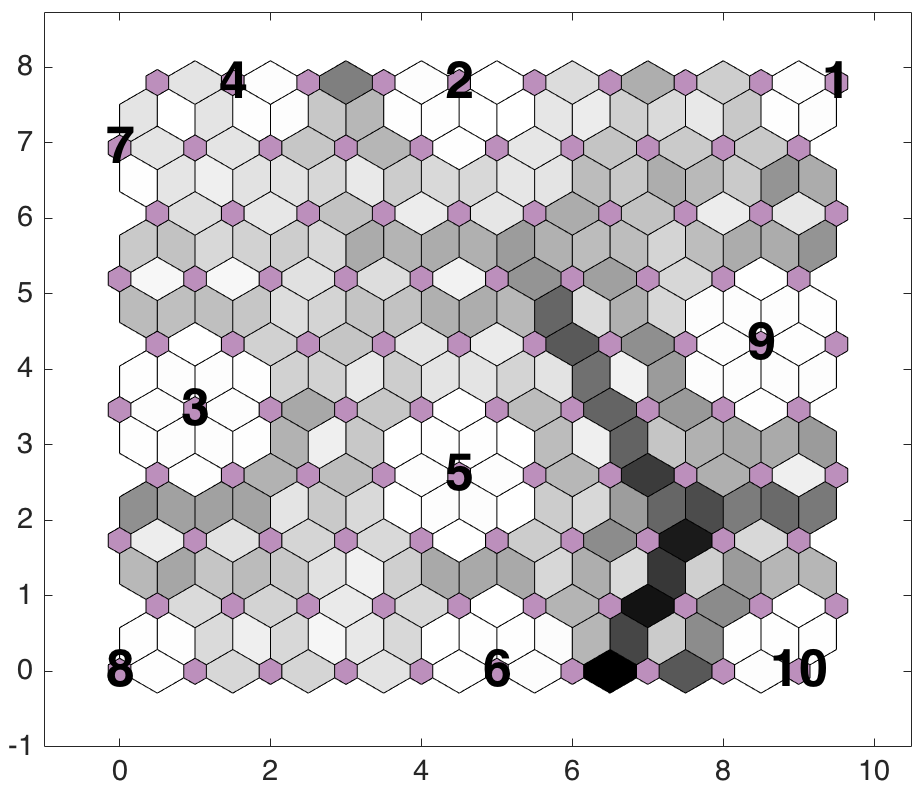
\includegraphics[width=0.5\textwidth]{../../images0.01/M31/2D/diff_dimension/combine_2D_data_between_cols3and26.png}
    \caption{Two-dimensional self-organizing map of M31 observations using a $10\times10$ grid. Similar to Figs.\ref{fig: sample} and \ref{fig: M31_nets_1d}, the hexagonal shapes show the neurons and the grey scale colours between neurons show the differences between weights of each neuron.}
    \label{fig: all_derived_ones}
\end{figure}
